
% \VignetteIndexEntry{An overview of the plot and stats functions in the surveyor package} 
% \VignettePackage{surveyor}
% \VignetteKeyword{surveyor}
% \VignetteKeyword{surveyor}


% Definitions
\newcommand{\surveyor}{\texttt{surveyor}}
\newcommand{\code}[1]{\texttt{#1}}
\newcommand{\ggplot}{\texttt{ggplot}}

\documentclass[10pt,oneside]{article}

\usepackage{Sweave}
\begin{document}
\pagestyle{empty}

\setlength{\baselineskip}{1.25em}
\setlength{\parskip}{0.5em}
\setlength{\parindent}{0.0em}



%\begin{titlepage}
\title{An overview of the plot and stats functions in the \surveyor{} package}
\author{Andrie de Vries}
%\end{titlepage}
\maketitle{}

\surveyor{} is a package that makes it easy to create graphical crosstabs from survey data files.  

%==============================================================================

\section{Introduction}

blah

%==============================================================================

\section{Create test data and a surveyor object}

\begin{Schunk}
\begin{Sinput}
> library(surveydata)
> library(surveyor)
> qData <- data.frame(
+     Q1 = c("Yes", "No", "Yes", "No", "Yes"),
+     Q2 = c(1, 1, 1, 0, 0),
+     Q3 = c("A", "B", "C", "B", "A"),
+     Q4_1 = c("Yes", "No", "Yes", "No", "Yes"), 
+     Q4_2 = c("Yes", "Yes", "No", "No", "Yes"), 
+     Q5_1 = c(1, 1, 1, 0, 0),
+     Q5_2 = c(0, 0, 1, 1, 1),
+     Q6_1 = c("A", "B", "C", "B", "A"),
+     Q6_2 = c("C", "B", "A", "B", "C"),
+     crossbreak = c("AAA", "AAA", "BBB", "BBB", "BBB"), 
+     crossbreak2 = c("DDD", "EEE", "DDD", "EEE", "DDD"),
+     weight = c(0.9, 1.1, 0.8, 1.2, 1.0)
+ )
> varlabels(qData) <- c(
+     "Single question with yes/no input", 
+     "Single question with binary input",
+     "Single question with multiple options",
+     "Multiple question with yes/no input: XX", 
+     "Multiple question with yes/no input: YY", 
+     "Multiple question with binary input: XX",
+     "Multiple question with binary input: YY",
+     "Multiple question with multiple options: XX",
+     "Multiple question with multiple options: YY",
+     "crossbreak",
+     "crossbreak2",
+     "weight")
> qData <- as.surveydata(qData)
\end{Sinput}
\end{Schunk}

Next, set up a surveyor object.  For the sake of illustrating the different options, we create to surveyor objects:
\begin{itemize}
\item sg: \surveyor{} object for \ggplot{} graphics
\item sl: \surveyor{} object for \code{lattice} graphics
\end{itemize}

\begin{Schunk}
\begin{Sinput}
> s <- as.surveyor(qData, qData$crossbreak, qData$weight)
> sg <- surveyorUpdateDefaults(s, outputToLatex = FALSE, addPlotTitle = TRUE)
> sl <- surveyorUpdateDefaults(sg, fastgraphics=TRUE)
> 
\end{Sinput}
\end{Schunk}

%==============================================================================

\section{Demonstrating the different plotBar options}

%--- plotBar with ggplot

\subsection{bar plots with ggplot}


\begin{Schunk}
\begin{Sinput}
> x <- plotBar(statsBin(codeGuess(sg, "Q1")))
> print(x$plot)
\end{Sinput}
\end{Schunk}
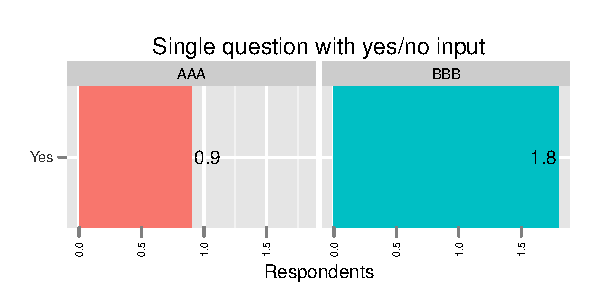
\includegraphics{graphics/figure-003}

\begin{Schunk}
\begin{Sinput}
> x <- plotBar(statsBin(codeGuess(sg, "Q2")))
> print(x$plot)
\end{Sinput}
\end{Schunk}
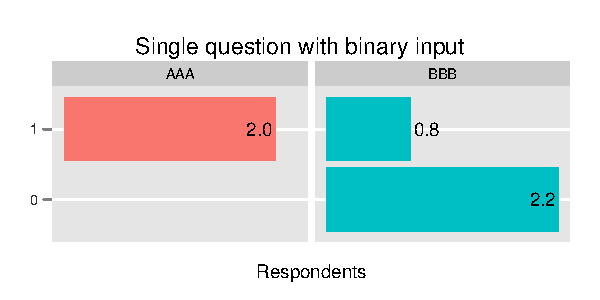
\includegraphics{graphics/figure-004}

\begin{Schunk}
\begin{Sinput}
> x <- plotBar(statsBin(codeGuess(sg, "Q3")))
> print(x$plot)
\end{Sinput}
\end{Schunk}
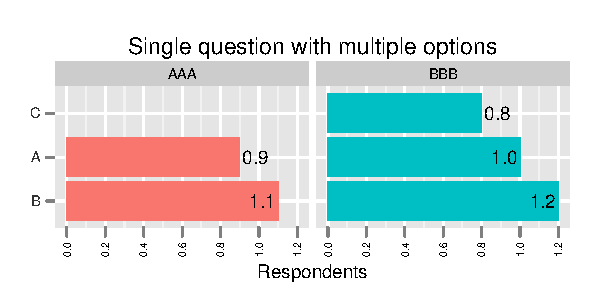
\includegraphics{graphics/figure-005}

\begin{Schunk}
\begin{Sinput}
> x <- plotBar(statsBin(codeGuess(sg, "Q4")))
> print(x$plot)
\end{Sinput}
\end{Schunk}
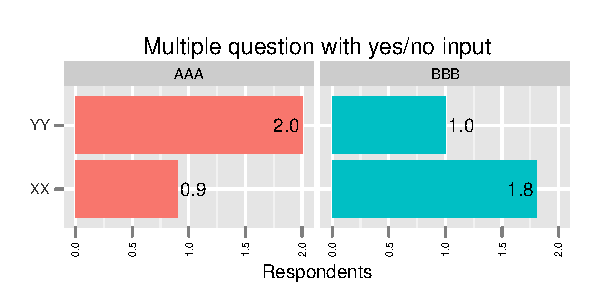
\includegraphics{graphics/figure-006}

\begin{Schunk}
\begin{Sinput}
> x <- plotBar(statsBin(codeGuess(sg, "Q5")))
> print(x$plot)
\end{Sinput}
\end{Schunk}
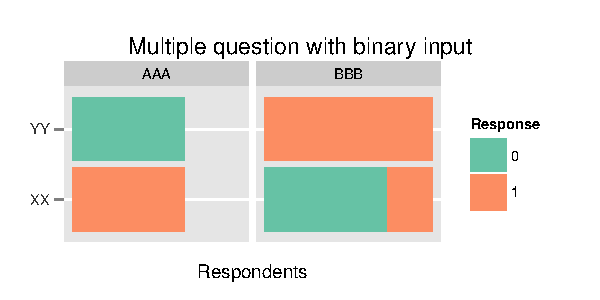
\includegraphics{graphics/figure-007}

\begin{Schunk}
\begin{Sinput}
> x <- plotBar(statsBin(codeGuess(sg, "Q6")))
> print(x$plot)
\end{Sinput}
\end{Schunk}
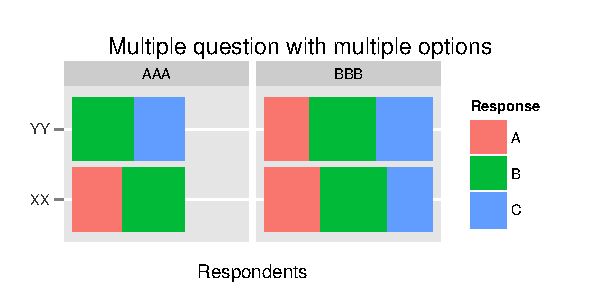
\includegraphics{graphics/figure-008}

%--- plotBar with lattice

\subsection{bar plots with lattice}


\begin{Schunk}
\begin{Sinput}
> x <- plotBar(statsBin(codeGuess(sl, "Q1")))
> print(x$plot)
\end{Sinput}
\end{Schunk}
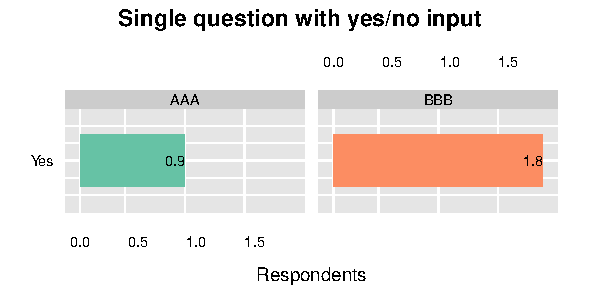
\includegraphics{graphics/figure-009}


\begin{Schunk}
\begin{Sinput}
> x <- plotBar(statsBin(codeGuess(sl, "Q2")))
> print(x$plot)
\end{Sinput}
\end{Schunk}
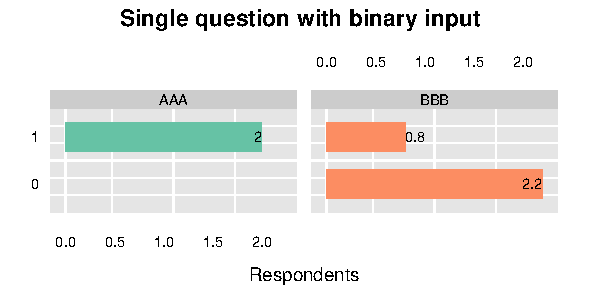
\includegraphics{graphics/figure-010}

\begin{Schunk}
\begin{Sinput}
> x <- plotBar(statsBin(codeGuess(sl, "Q3")))
> print(x$plot)
\end{Sinput}
\end{Schunk}
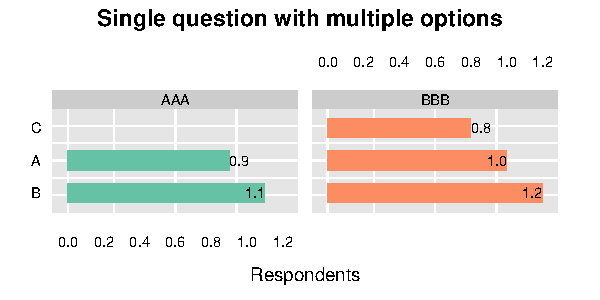
\includegraphics{graphics/figure-011}

\begin{Schunk}
\begin{Sinput}
> x <- plotBar(statsBin(codeGuess(sl, "Q4")))
> print(x$plot)
\end{Sinput}
\end{Schunk}
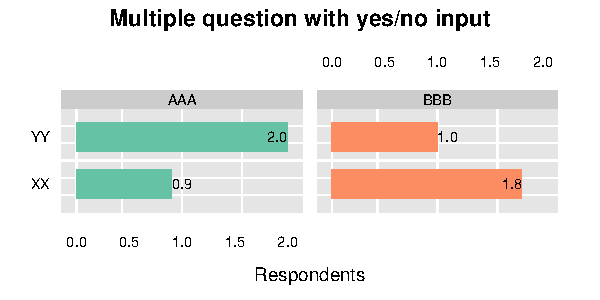
\includegraphics{graphics/figure-012}

\begin{Schunk}
\begin{Sinput}
> x <- plotBar(statsBin(codeGuess(sl, "Q5")))
> print(x$plot)
\end{Sinput}
\end{Schunk}
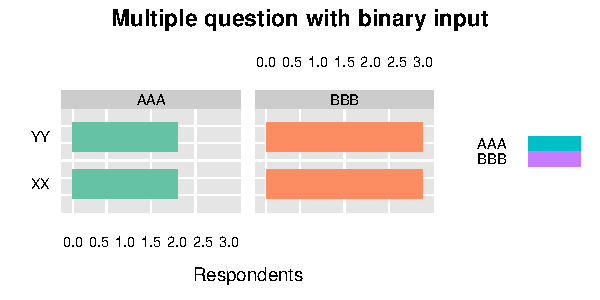
\includegraphics{graphics/figure-013}

\begin{Schunk}
\begin{Sinput}
> x <- plotBar(statsBin(codeGuess(sl, "Q6")))
> print(x$plot)
\end{Sinput}
\end{Schunk}
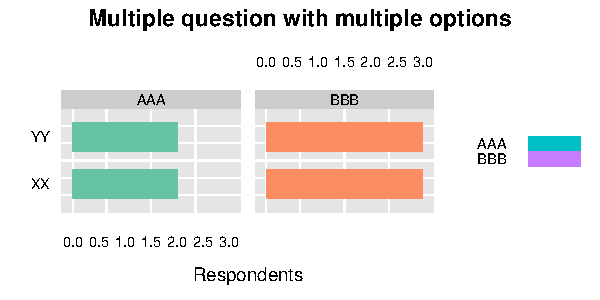
\includegraphics{graphics/figure-014}

%==============================================================================

\section{Demonstrating the different plotColumn options}

%--- plotColumn with ggplot

\subsection{Column plots with ggplot}


\begin{Schunk}
\begin{Sinput}
> x <- plotColumn(statsBin(codeGuess(sg, "Q1")))
> print(x$plot)
\end{Sinput}
\end{Schunk}
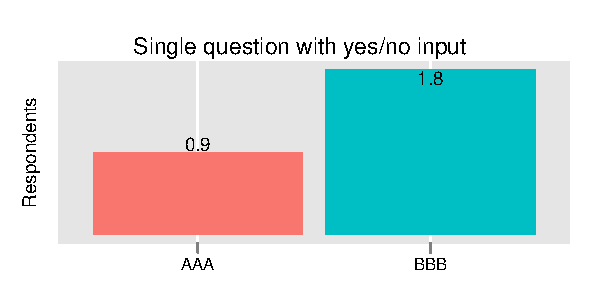
\includegraphics{graphics/figure-015}

\begin{Schunk}
\begin{Sinput}
> x <- plotColumn(statsBin(codeGuess(sg, "Q2")))
> print(x$plot)
\end{Sinput}
\end{Schunk}
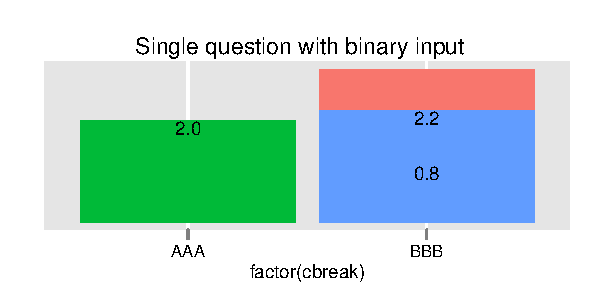
\includegraphics{graphics/figure-016}

\begin{Schunk}
\begin{Sinput}
> x <- plotColumn(statsBin(codeGuess(sg, "Q3")))
> print(x$plot)
\end{Sinput}
\end{Schunk}
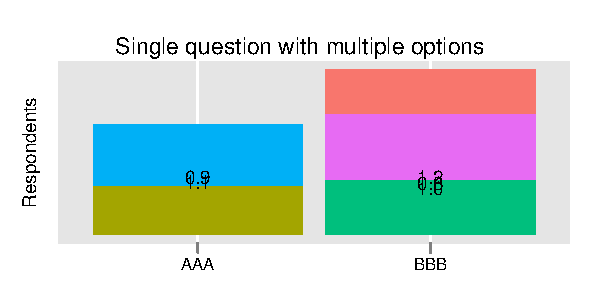
\includegraphics{graphics/figure-017}

\begin{Schunk}
\begin{Sinput}
> x <- plotColumn(statsBin(codeGuess(sg, "Q4")))
> print(x$plot)
\end{Sinput}
\end{Schunk}
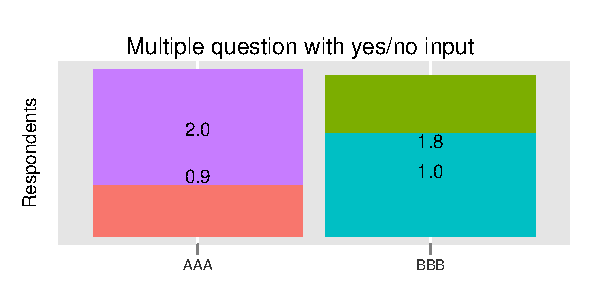
\includegraphics{graphics/figure-018}

\begin{Schunk}
\begin{Sinput}
> x <- plotColumn(statsBin(codeGuess(sg, "Q5")))
> print(x$plot)
\end{Sinput}
\end{Schunk}
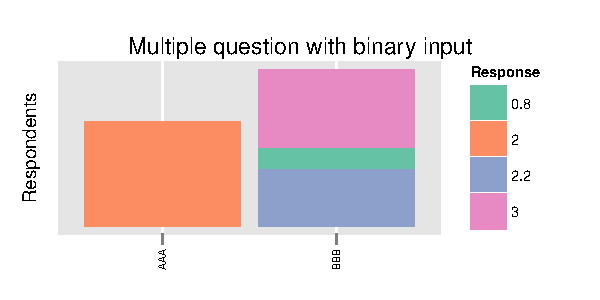
\includegraphics{graphics/figure-019}

\begin{Schunk}
\begin{Sinput}
> x <- plotColumn(statsBin(codeGuess(sg, "Q6")))
> print(x$plot)
\end{Sinput}
\end{Schunk}
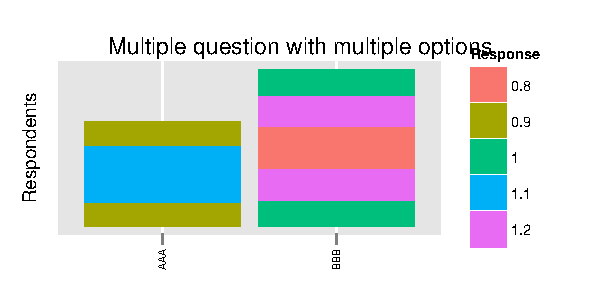
\includegraphics{graphics/figure-020}

%--- plotColumn with lattice

\subsection{Column plots with lattice}


\begin{Schunk}
\begin{Sinput}
> x <- plotColumn(statsBin(codeGuess(sl, "Q1")))
> print(x$plot)
\end{Sinput}
\end{Schunk}
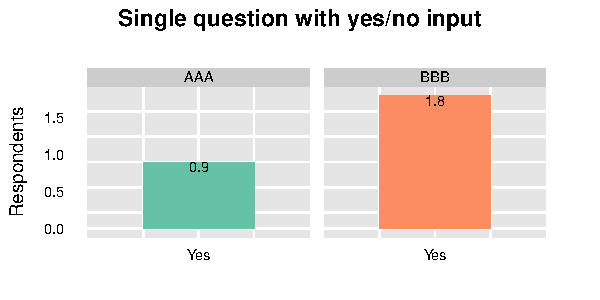
\includegraphics{graphics/figure-021}


\begin{Schunk}
\begin{Sinput}
> x <- plotColumn(statsBin(codeGuess(sl, "Q2")))
> print(x$plot)
\end{Sinput}
\end{Schunk}
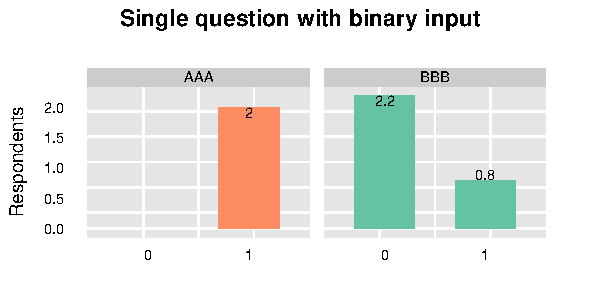
\includegraphics{graphics/figure-022}

\begin{Schunk}
\begin{Sinput}
> x <- plotColumn(statsBin(codeGuess(sl, "Q3")))
> print(x$plot)
\end{Sinput}
\end{Schunk}
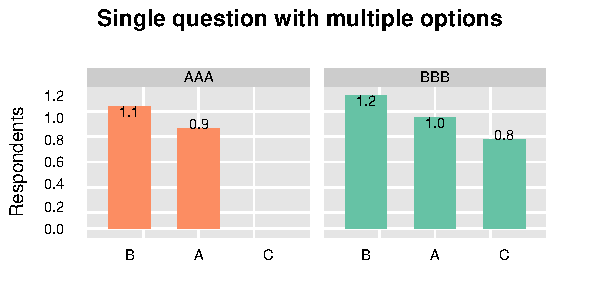
\includegraphics{graphics/figure-023}

\begin{Schunk}
\begin{Sinput}
> x <- plotColumn(statsBin(codeGuess(sl, "Q4")))
> print(x$plot)
\end{Sinput}
\end{Schunk}
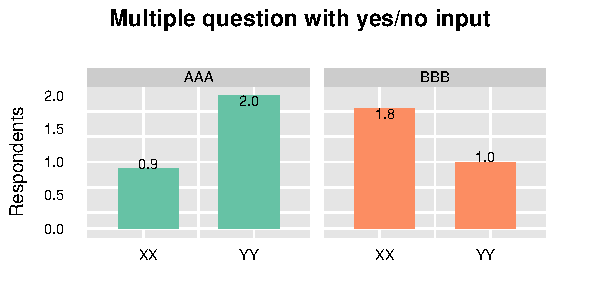
\includegraphics{graphics/figure-024}

\begin{Schunk}
\begin{Sinput}
> x <- plotColumn(statsBin(codeGuess(sl, "Q5")))
> print(x$plot)
\end{Sinput}
\end{Schunk}
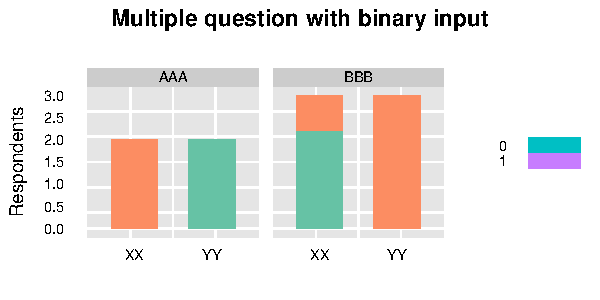
\includegraphics{graphics/figure-025}

\begin{Schunk}
\begin{Sinput}
> x <- plotColumn(statsBin(codeGuess(sl, "Q6")))
> print(x$plot)
\end{Sinput}
\end{Schunk}
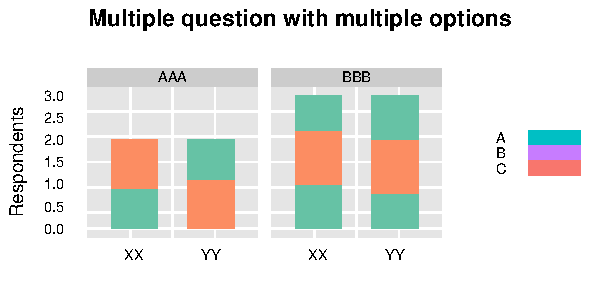
\includegraphics{graphics/figure-026}


\section{Conclusion}

The \surveyor{} packages makes it easy to analyse survey data files.

% Start a new page
% Not echoed, not evaluated
% ONLY here for checkVignettes so that all output doesn't
% end up on one enormous page

\end{document}




